\subsection{The ALICE Detector}
\begin{itemize}
    \item What is the LHC?
    \item What is ALICE?
    \item What does ALICE look for?
    \item What is Run 3?
\end{itemize}
The ALICE detector (A Large Ion Collider Experiment) is a detector experiment at the Large Hadron Collider (LHC) at CERN. Its primary goal is the investigation of ``strongly interacting matter at extreme energy densities, where a formation of a new phase of matter, the quark-gluon plasma, is expected'' (\cite{ALICE_LOI}). It achieves this goal by studying the products of head-on collisions of heavy ions such as lead. 

% ALICE is situated at 

% The LHC at CERN in Geneva is built to accelerate particles up to very high energies (\SI{13.6}{\tera\electronvolt})

The coordinate system used at ALICE needs to be discussed first in order to fully explain the scope of this report. A modified cylindrical coordinate system is used as most detectors in the experiment are cylindrically symmetric about the beamline of the LHC. We place the $z$-axis along the beamline and call the angle around the $z$-axis $\varphi$, the azimuthal angle. The angle from the $z$-axis to the $x-y$ plane is called $\theta$, the polar angle. 
We are interested in the momentum of particles that we track in the detector, which we call $\vec{p}$, but we also define the transverse momentum $p_{\mathrm{T}}=\sqrt{p_x^2 + p_y^2}$. The last important coordinate to discuss is the rapidity, often denoted as $y$. This is defined as 
\begin{equation}
    y=\frac 12 \ln\left(\frac{E+p_z}{E-p_z}\right)
    \label{eqn:rapidity}
\end{equation}
where $E$ is the total energy of the particle being considered

\begin{figure}[h]
    \begin{center}
        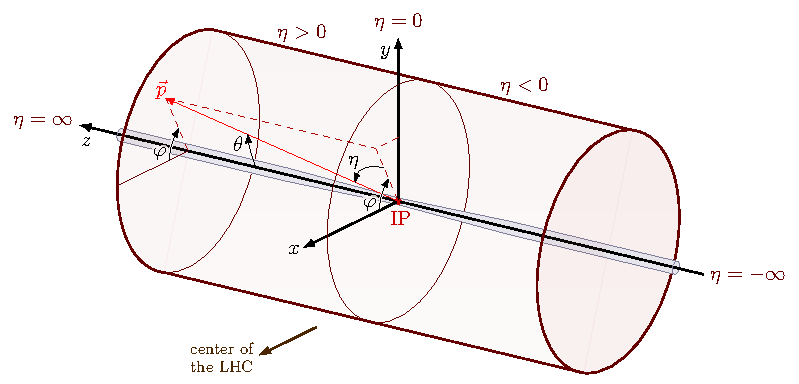
\includegraphics[width=.8\textwidth]{Figs/coords.pdf}
        \caption{Coordinate system \cite{coords}}
        \label{fig:coords}
    \end{center}
\end{figure}


\subsection{Run 3 Specifics}
\begin{itemize}
    \item What was upgraded/added in Run 3?
    \item 
\end{itemize}

\subsection{Muon Forward Tracker}